% 东华大学硕士学位毕业论文
% 基于多尺度状态空间模型和自适应频域滤波的医学图像分割
%%%%%%%%%%%%%%% 导入风格包 %%%%%%%%%%%%%%%
\documentclass[12pt, a4paper, twoside]{article}
\usepackage{dhuMaster/resume/dhuMasterstyle}

%%%%%%%%%%%%%%% 论文主题 %%%%%%%%%%%%%%%
\begin{document}
\pagenumbering{Roman}

%%%%%%%%%%%%%%% 中文题目与摘要 %%%%%%%%%%%%%%%
\reTitle{基于多尺度状态空间模型和自适应频域滤波的医学图像分割}
\reAbstract

医学图像分割是现代精准医疗与计算机辅助诊断中的关键技术，其精度直接影响临床诊疗决策。然而，医学图像中普遍存在的目标尺度多样性以及边界模糊、信息丢失等问题，严重制约了现有分割方法的性能。针对上述挑战，本文提出了SAF-Mamba模型，该模型结合多尺度视觉状态空间（Multi-Scale Visual State Space, MSVSS）模块与自适应滤波器模块（Adaptive Filter Block, AFB），分别应对尺度变化与边界细化两大核心难题。MSVSS模块通过并行多尺度深度卷积分支、通道整合与校准机制，有效捕获不同尺度目标的特征表示；AFB模块则利用自适应滤波器生成器（AF Generator）在频域中动态调制特征，增强边界细节的保留。在ACDC心脏磁共振数据集上，本文方法取得了92.21\%的Dice相似系数（Dice Similarity Coefficient, DSC）和1.05 mm的95\%豪斯多夫距离（95\% Hausdorff Distance, HD95）；在M\&Ms多中心、多厂商心脏分割数据集上，取得了88.43\%的DSC和12.14 mm的HD95，均优于基于卷积神经网络（Convolutional Neural Network, CNN）、Transformer及Mamba的现有方法，验证了本文方法的有效性与泛化能力。

\reKeyword{医学图像分割；Mamba；状态空间模型；多尺度特征；自适应频域滤波}

%%%%%%%%%%%%%%% 英文题目与摘要 %%%%%%%%%%%%%%%
\reTitleEN{Medical Image Segmentation Based on Multi-Scale Mamba and Adaptive Frequency Filtering}
\reAbstractEN

Medical image segmentation is a key technology in modern precision medicine and computer-aided diagnosis, and its accuracy directly affects clinical decision-making. However, the widespread problems of target scale diversity, boundary blurring, and information loss in medical images seriously restrict the performance of existing segmentation methods. To address these challenges, this thesis proposes the SAF-Mamba model, which combines the Multi-Scale Visual State Space (MSVSS) module and the Adaptive Filter Block (AFB) to tackle the two core problems of scale variation and boundary refinement. The MSVSS module effectively captures feature representations of targets at different scales through parallel multi-scale depth-wise convolution branches, channel integration, and calibration mechanisms. The AFB module uses an Adaptive Filter Generator to dynamically modulate features in the frequency domain, enhancing the preservation of boundary details. On the ACDC cardiac MRI dataset, the proposed method achieves a Dice Similarity Coefficient (DSC) of 92.21\% and a 95\% Hausdorff Distance (HD95) of 1.05 mm. On the M\&Ms multi-center, multi-vendor cardiac segmentation dataset, it achieves 88.43\% DSC and 12.14 mm HD95, outperforming existing CNN-based, Transformer-based, and Mamba-based methods, validating the effectiveness and generalization capability of the proposed approach.

\reKeywordEN{Medical image segmentation; Mamba; State space model; Multi-scale features; Adaptive frequency filtering}

%%%%%%%%%%%%%%% 目录 %%%%%%%%%%%%%%%
\begin{center}
    \tableofcontents
\end{center}

%%%%%%%%%%%%%%% 第一章 绪论 %%%%%%%%%%%%%%%
\reSection{第一章\quad 绪论}
\pagenumbering{arabic}

本章首先阐述医学图像分割的研究背景及意义，接着对国内外研究现状进行系统性梳理，并介绍本文的研究目标与主要内容，最后概述全文的组织结构。

\subsection{研究背景及意义}

国务院办公厅印发的《“十四五”国民健康规划》明确指出：“要把保障人民健康放在优先发展的战略位置，全面推进健康中国建设是实现中华民族伟大复兴的重要基础”[1]。随着国家对国民健康事业的高度重视以及人民健康意识的持续提升，医学影像技术作为现代医学的重要组成部分，正迎来前所未有的发展机遇。以磁共振成像（Magnetic Resonance Imaging, MRI）、计算机断层扫描（Computed Tomography, CT）、X射线（X-ray）以及超声（Ultrasound, US）为代表的高端成像设备，如图1.1中呈现的不同医学影像技术所示，它们使得医生能够以非侵入式、直观且高清晰度的方式探查人体内部复杂的解剖结构与潜在病灶。这不仅显著提高了疾病诊断的准确性，也为各类重大疾病的提早甄别与干预争取了极为宝贵的治疗时间[2]。

然而，随着高分辨率医疗设备的加速普及，医学影像数据呈现出爆炸式增长。传统的人工分析方法依赖资深放射科医师进行人工阅片与影像判读，逐渐暴露出分析效率受限、精度易受主观经验与视觉疲劳干扰等问题[3]。特别是面对复杂多变且对比度较低的软组织图像时，专家人工评估的可靠性和一致性面临着巨大挑战。随着计算机技术的不断进步，早期基于图像处理与数学模型的计算机辅助诊断方法开始进入医学影像分析领域，在一定程度上缓解了人工阅片的压力。然而，这类方法依赖手工设计的特征与规则，面对结构复杂、变异多端的真实临床数据，泛化能力有限。近年来，深度学习凭借其自动特征学习能力，逐渐成为医学影像智能化分析的主流技术路线，推动了图像分割精度与自动化程度的大幅提升。

自动医学图像分割是医学图像分析中一个关键的研究领域。其主要目标在于利用计算机视觉技术，从复杂的扫描背景中识别并剥离出感兴趣区域，如：解剖结构、特定脏器或病理组织等，从而为后续的体积测量、病理性质分析及三维重建等奠定像素级的基础。作为现代精准医疗与计算机辅助诊断的核心环节，其临床应用价值主要体现在以下三个维度：

精准诊断：自动图像分割能够帮助医生从混杂的解剖背景中定量提取出器官与病变区域。通过精确测量病灶在三维或二维空间的体积、形态和拓扑结构，能够大幅提升病理判断分期的客观性与可靠性。
治疗规划：在放射治疗或外科手术干预的筹备阶段，术前精确描绘的病变靶区能够为医疗机器人或放疗系统提供三维“导航图”。这要求算法不仅能在摧毁恶性组织的同时最大程度避开周围正常脏器以减少副作用，更直接关系到患者的生存质量。
术后监测：通过对患者随访周期的海量影像进行连续自动化分割，医生能够高频度、定量化追踪病灶的变化轨迹（如复发、缩小或向周围组织浸润）。这对于动态调整化疗靶向方案及客观评估预后疗效具有高度的科学依据价值。
尽管深层人工神经网络在自动化医学图像分割领域取得了突破性进展，但在真实世界高度复杂的临床场景中，当前主流的视觉预测算法依然面临着两大长期悬而未决的共性学术难题：

第一，目标尺度多样性挑战。人体的形态解剖学结构极其复杂，即便获取自同一成像设备、身处同一张医学切片中，不同解剖部位或病灶的物理尺寸也常常存在跨越数量级的悬殊差异。例如，在心脏磁共振图像中，左右心室腔的广阔区域与纤薄微小的心肌壁形成了强烈的尺度对比；而在皮肤显微图像中，早期细小溃疡与晚期弥散性红斑也常常共处于同一视野。现有的多种深层网络模型在特征提取阶段，往往受限于单一且固定的感受野，缺乏显式的跨尺度融合感知机制。这直接导致算法在微小靶区极易发生结构性漏分或像素断裂，而在大面积靶区则易受到局部杂讯干扰从而丢失整体的拓扑连贯性。

第二，边界高频信息丢失与组织粘连挑战。受限于软组织相近的物理射线吸收率或磁共振弛豫时间，加之受限于成像设备的固有热噪声与伪相分辨率，医学影像中许多关键器官或病灶的边缘往往呈现出严重模糊甚至与毗邻组织大面积粘连的表象。更为致命的是，目前主流的图像深度学习模型，为了提取全局高阶语义特征同时压缩空间计算量，普遍采用逐层池化或带有步幅的大核卷积来进行特征下采样。这一信号降频过程，会以不可逆的方式物理级抹除并抛弃蕴藏着图像纹理及其边缘几何形状的高频有效特征。当网络在解码重建阶段试图仅凭残留的低频语义来还原受损的高频空间信息时，往往心有余而力不足。最终输出的预测掩码在边缘处不够紧密贴合真实解剖结构，伴随着令人难以接受的锯齿和粗糙过平滑伪影，这在容错率极低的临床应用场景中是无法接受的。

综上所述，针对医学图像分割任务中长久存在的目标尺度多样性与边界高频特征丢失这两大顽固痛点，探索并设计一种同时兼顾大感受野多尺度捕捉能力以及具备频域自适应高频边界增强约束的新型网络框架，具有十分重要的前沿理论探索价值和迫切的临床落地需求。

\subsection{国内外研究现状}

医学图像分割技术的发展经历了从传统算法到深度学习方法的演进。本节对相关技术进行系统性梳理，为后文提出的方法奠定研究坐标。

\subsubsection{基于传统方法的医学图像分割技术}


传统分割技术在很长一段时间内一直是医学图像分析的基础，这些方法主要依赖于预定义的规则和图像强度。传统方法的优势在于其较高的计算效率与可解释性，但在处理包含高噪声、剧烈强度变化或边界模糊的复杂医学图像时，其性能往往会受到限制。根据现有文献的分类，传统医学图像分割方法主要可分为以下五大类：

阈值分割技术 (Thresholding Techniques) 的核心是将灰度图像转换为二值图像，通过设定阈值将像素划分为目标前景或背景。阈值分割主要分为全局阈值法和局部阈值法两种。全局阈值法使用单一、恒定的阈值，适用于前景与背景灰度分布差异明显的图像，经典算法包括通过最大化类间方差来寻找最佳阈值的Otsu法、迭代阈值法、最小误差阈值法（Kittler-Illingworth法）以及基于熵的阈值法。然而，全局阈值法对于由阴影或定向光照等因素导致的光照不均的复杂场景效果不佳，这种情况下可以采用局部阈值法。局部算法通过分析每个像素局部邻域内的统计特征，如亮度、对比度等，来动态分配阈值，代表性方法包括Niblack算法、在低纹理背景下对Niblack法进行了改进的Sauvola算法以及利用局部对比度区分高低对比度区域的Bernsen算法。

基于边缘的分割 (Edge-Based Segmentation) 方法也是一种直观的方式。边缘是两个同质区域之间的边界，表现为图像亮度的局部变化。基于边缘的分割通常包括图像预处理、边缘检测、非极大值抑制、阈值化以及后处理等步骤。该方法广泛使用一阶或二阶微分算子来提取边缘的梯度或曲率信息。常见的一阶微分算子包括Roberts算子、Prewitt算子、Sobel算子和Canny算子。其中，Roberts算子计算简单、速度快，但对噪声极为敏感；Prewitt和Sobel算子对邻域像素进行差分，具有较好的噪声抑制能力；Canny算子则通过多阶段处理实现了高精度的边缘定位和出色的噪声抑制，但计算复杂度较高。二阶微分算子对图像细节敏感，通常结合高斯平滑来缓解噪声的干扰，用来实现更精确的边缘定位。

基于区域的分割方法 (Region-Based Segmentation) 主要依赖于像素在颜色、亮度、纹理间的相似性以及空间邻近性，将图像划分为具有相似属性的多个区域。其中最主要的算法有种子区域生长法（Seeded Region Growing, SRG）和分裂合并法（Split and Merge）。

聚类分割 (Clustering-Based Segmentation) 旨在将具有相似特征的像素归入同一簇中，使位于同一簇内的元素相似度最大化，不同簇之间的差异性最大化。聚类方法可划分为层次聚类（Hierarchical Clustering）和划分聚类（Partitional Clustering）。层次聚类通过构建自底向上的凝聚型或自顶向下的分裂型树状图（树状结构）来完成聚类。但层次聚类采用贪心策略，一旦分配便无法纠正，且不优化任何目标函数，较高的时间复杂度在处理高维医学图像时面临极大挑战。划分聚类则通过优化目标函数来最小化簇内相似度。常见的划分聚类算法包括软聚类（如模糊C均值聚类，FCM）和硬聚类（如K均值算法）。划分聚类能够迭代提升聚类质量，但对初始条件、噪声以及异常值较为敏感。

基于图的分割方法 (Graph-Based Segmentation) 将图像映射为图结构，其中顶点代表图像像素或区域，边代表相邻顶点间的关系，边的权重用于量化顶点间的某种属性或相似度,。图像分割即转化为图的划分问题。主要的技术包括最小生成树（MST，如Kruskal和Prim算法）和图割法（Graph Cuts）。在图割法中，图像被转换为包含源节点和汇节点的s-t图，并通过n-links（邻域像素间）和t-links（终端节点间）来评估像素归属，具体衍生出最小割、归一化割（Ncut）等多种代价函数优化策略,,。此外，该领域还包括马尔可夫随机场（MRF，通过最大后验概率估计进行像素标记并融入局部先验信息）以及最短路径方法（如Dijkstra或Bellman-Ford算法）。

综上所述，传统医学图像分割技术通过明确的数学模型与规则，为疾病诊断和治疗规划提供了重要的早期解决方案。然而，面对现代医学成像中普遍存在的噪声干扰、边界模糊以及复杂的个体异质性，传统方法难以应对。这一局限性也为后续基于深度学习的自动化特征提取技术的崛起提供了明确的驱动力。

\subsubsection{基于深度学习的医学图像分割技术}

深度学习直接从数据中学习到重要的结构和其内在联系的特征，并使用端到端的方式将结果进行呈现，因为更快的处理速度和更高的分割精度而成为了目前的主流方法。其在语义分割领域的突破是由于全卷积网络（Fully Convolutional Networks, FCN）的提出。卷积神经网络（CNN）由于在网络末端使用全连接层进行图像级分类而导致空间信息的丢失，针对这一问题FCN开创性地移除了全连接层，使网络能够接收任意尺寸的图像并输出像素级别的密集预测，解决了语义分割的核心问题。在FCN的基础上，Ronneberger等人于2015年提出的专门针对医学图像的U-Net模型确立了医学图像分割中经典的编码器-解码器（Encoder-Decoder）范式。U-Net引入了跳跃连接（Skip Connections），它将编码器中包含丰富空间定位信息的浅层特征，直接与解码器中包含高级语义信息的深层特征进行拼接融合。这种设计有效弥补了下采样过程中的空间信息丢失，使得模型在有限的医学标注数据上也能实现精准的边缘定位和目标分割。

随着医学图像任务复杂度的增加，在U-Net的基础上衍生出了两大主流改进方向，即基于CNN的改进模型与基于Transformer的模型。UNet++在U-Net的基础上引入了嵌套的U型结构和密集跳跃连接，允许网络在不同的深度和尺度上聚合特征，从而有效缩小了编码器和解码器之间的语义鸿沟。此外，为了让模型更加关注病灶区域，Attention U-Net在跳跃连接中引入了注意力门，使网络能够隐式地抑制无关的背景区域，同时突出显示与分割任务高度相关的感兴趣区域。尽管这些CNN变体性能优异，但由于卷积操作固有的感受野受限问题，它们难以对图像中的长距离像素建立依赖关系和全局上下文建模。为了克服CNN感受野的局限性，具有全局建模能力的Transformer被引入医学视觉领域。TransUNet构建了CNN与Transformer的混合编码器，这种设计既保留了CNN的局部纹理感知力，又弥补了长距离建模的不足。随后提出的Swin-Unet则构建了首个纯Transformer的U型架构，摒弃了卷积操作，使用具有层次化结构的Swin Transformer作为主干，并通过移位窗口机制在局部窗口内计算自注意力，在捕获全局特征的同时降低了传统Transformer的计算复杂度。尽管Transformer在全局建模上具有显著优势，但其模型中核心的自注意力机制的计算复杂度会随着图像空间分辨率呈平方级增长。这导致其在处理高分辨率或3D医学图像时面临极高的计算开销和内存消耗瓶颈。

为了解决CNN局部感受野受限以及Transformer计算复杂度过高的问题，状态空间模型（State Space Models, SSMs），特别是最新的Mamba架构，正作为一种新兴的序列建模方法在视觉任务中受到广泛关注。Mamba模型在结构化状态空间模型（Structured State Space Model, S4）的基础上引入了输入依赖的动态选择机制（Selection Mechanism）和硬件感知（Hardware-aware）的并行扫描算法，实现了线性复杂度的长序列建模。VMamba将Mamba扩展至视觉任务，提出视觉状态空间（Visual State Space, VSS）模块，通过多方向扫描策略缓解一维序列与二维图像之间的方向敏感性。在医学图像分割领域，器官或病灶往往跨越极大的空间范围，Mamba的出现完美契合了医学图像对高分辨率和全局上下文的双重需求。Mamba-UNet将VSS模块嵌入U-Net架构，在医学图像分割任务上展现出优异性能。Mamba为解决复杂医学图像分割提供了一个极具前景的新型基座架构，本研究在Mamba-Unet的基础上开展了进一步的探索。


\subsection{研究目标及内容}

针对医学图像分割中的尺度变化与边界模糊两大挑战，本文的研究目标是设计一个基于状态空间模型的高效、通用分割框架，并完成以下研究内容：

（1）设计多尺度视觉状态空间（MSVSS）模块，通过并行多尺度深度卷积分支、通道整合与校准机制，捕获不同尺度目标的特征表示，增强模型对尺度变化的敏感性。

（2）构建自适应滤波器模块（AFB），利用快速傅里叶变换（Fast Fourier Transform, FFT）将特征映射至频域，通过自适应滤波器生成器动态调制频率分量，增强边界细节并抑制噪声，最后经逆傅里叶变换（Inverse FFT, IFFT）重构空间特征。

（3）将MSVSS与AFB集成于U型编码器-解码器架构，形成完整的SAF-Mamba网络，在编码器各阶段嵌入MSVSS模块，在跳跃连接中引入AFB模块。

（4）在ACDC、M\&Ms等公开心脏分割数据集上进行实验，通过对比实验、消融实验与可视化分析，验证方法的有效性与泛化能力。

\subsection{本文的组织结构}

本文共分为五章，各章内容安排如下：

第一章为绪论，阐述医学图像分割的研究背景、意义及国内外研究现状，并明确研究目标与内容。

第二章介绍相关理论与技术基础，包括卷积神经网络、状态空间模型与频域图像分析理论，为后续方法章节提供理论铺垫。

第三章详细阐述基于多尺度状态空间模型的医学图像分割方法，包括MSVSS模块的设计与SA-Mamba网络架构，并在心脏数据集上进行实验验证。

第四章介绍基于自适应频域滤波的边界细化方法，包括AFB模块的设计原理与实现细节，通过消融实验与泛化实验验证SAF-Mamba的综合性能。

第五章对全文工作进行总结，并展望未来研究方向。

%%%%%%%%%%%%%%% 第二章 相关理论与技术基础 %%%%%%%%%%%%%%%
\reSection{第二章\quad 相关理论与技术基础}

本章为后续方法章节中出现的所有关键技术概念提供详尽的理论铺垫，包括卷积神经网络基础、状态空间模型理论以及频域图像分析理论。

\subsection{卷积神经网络基础}


卷积神经网络（Convolutional Neural Networks, CNNs）是计算机视觉领域，尤其是语义分割任务中的核心基石。从生物学视角来看，CNN 的构建受自然视觉感受机制的启发，特别是 Hubel 和 Wiesel 对动物视觉皮层接收区光线检测功能的研究，为模拟人类视觉感知的层级化处理奠定了生物学基础。CNN 的基本结构包括卷积层、池化层、激活函数和损失函数，以及反向传播机制。

\textbf{（1）卷积层（Convolutional Layer）}

卷积操作是神经网络提取特征表征的核心手段，其本质是通过滑动窗口机制与权重共享策略，在输入特征图上实现局部空间特征的函数映射。在医疗影像分割等高精度需求场景下，卷积变体的选择与设计直接影响模型对解剖结构边界的捕获能力。设输入特征图为$\mathbf{X} \in \mathbb{R}^{H \times W \times C}$，卷积核为$\mathbf{K} \in \mathbb{R}^{k \times k \times C}$，则卷积操作可表示为：


\begin{equation}
\mathbf{Y}(i,j) = \sum_{m,n} \mathbf{K}(m,n) \cdot \mathbf{X}(i+m, j+n)
\end{equation}
不同尺寸的卷积核对应不同的感受野，$k \times k$卷积核的感受野为$k \times k$像素。感受野决定了网络每一层输出特征图上的像素点在原图上映射的区域大小，是理解多尺度特征提取的关键概念。常规卷积依靠局部连接与空间权重共享，能够高效捕获图像中的纹理、边缘等空间特征，实现特征提取的平移不变性。转置卷积（Transposed Convolution）作为实现上采样的关键手段，通过建立一对多的映射关系恢复特征分辨率，然而由于在计算中对输入矩阵进行填零扩大，核函数在滑动过程中往往产生非均匀重叠，导致输出图像出现明显的"棋盘效应"（Checkerboard Effect），在医疗影像中常表现为类间边界的锯齿状伪影，限制了边缘分割精度。空洞卷积（Dilated Convolution）通过引入扩张率（Dilation Rate）扩大感受野，能够在不增加参数负担的前提下捕捉多尺度上下文信息，但过大的扩张率会导致"网格效应"（Gridding Effect），造成局部像素相关性的丢失。可变形卷积（Deformable Convolution）针对标准卷积核固定几何形状的局限，通过学习额外的偏移量（Offset）来动态调整采样位置，对医疗影像中形状极不规则的组织器官或病灶边界展现了更强的建模灵活性，显著提升了复杂语义边界的拟合能力。深度可分离卷积（Depth-wise Separable Convolution）将标准卷积分解为逐通道卷积与逐点卷积，在保持表达能力的同时显著降低参数量与计算量，被广泛应用于MobileNet、EfficientNet等轻量化架构中，亦为本文MSVSS模块中并行多尺度深度卷积的设计提供了效率保障。

\textbf{（2）池化层（Pooling Layer）}

池化层作为典型的下采样操作，其战略职能在于压缩特征图的空间维度，在减少参数冗余的同时，维持网络对输入信号在平移与尺度上的鲁棒性。设局部感受野窗口为$\mathcal{R}_{i,j}$，最大池化与平均池化分别定义为：
\begin{equation}
\mathbf{P}_{\max}(i,j) = \max_{(m,n)\in\mathcal{R}_{i,j}} \mathbf{X}(m,n)
\end{equation}
\begin{equation}
\mathbf{P}_{\text{avg}}(i,j) = \frac{1}{|\mathcal{R}_{i,j}|} \sum_{(m,n)\in\mathcal{R}_{i,j}} \mathbf{X}(m,n)
\end{equation}
最大池化侧重于提取局部区域内最显著的判别性特征，适用于识别高亮或明显的组织特征；平均池化则更倾向于保留整体背景的统计特性，维持语义信息的平滑性。借鉴 Dropout 的正则化思想，混合池化通过随机切换池化策略增强网络的泛化表现；随机池化则基于元素值的大小设定选取概率，确保非显著特征也有贡献权重的可能，有效缓解过拟合现象。池化后的特征需经非线性激活函数（如 ReLU、Softmax 等）转换，以构建复杂的非凸决策边界，最终由损失函数量化模型预测与真实标签之间的偏差。

\textbf{（3）损失函数（Loss Function）}

损失函数作为量化指标，直接定义了模型参数优化的目标空间，指导梯度下降算法的演进方向。均方误差（Mean Squared Error, MSE）通过计算预测值与真实值差值的平方和来衡量偏差，设预测值为$\hat{y}_i$、真实值为$y_i$，其定义为：
\begin{equation}
\mathcal{L}_{\text{MSE}} = \frac{1}{N}\sum_{i=1}^{N}\left(\hat{y}_i - y_i\right)^2
\end{equation}
其数学性质优良，有利于梯度平滑收敛，但平方项的权重分配使其对离群点（Outliers）极度敏感，容易导致训练过程受极端样本干扰。交叉熵损失（Cross Entropy, CE）基于信息论背景，设$p_i$为真实分布、$q_i$为预测概率分布，其定义为：
\begin{equation}
\mathcal{L}_{\text{CE}} = -\sum_{i=1}^{C} p_i \log q_i
\end{equation}
CE 衡量了预测概率分布与真实分布之间的 KL 散度，在语义分割等多分类任务中与 Softmax 函数耦合使用时展现出显著的收敛优势，能够有效避免梯度饱和现象，是目前像素级密集预测任务的主导损失函数。

\textbf{（4）反向传播（Backpropagation）}

反向传播算法是神经网络实现自我进化的核心逻辑，其运行基于多元复合函数求导的链式法则。设网络第$l$层的损失梯度为$\delta^{(l)}$，则链式法则给出：
\begin{equation}
\delta^{(l)} = \frac{\partial \mathcal{L}}{\partial \mathbf{z}^{(l)}} = \left(\mathbf{W}^{(l+1)\top} \delta^{(l+1)}\right) \odot \sigma'\!\left(\mathbf{z}^{(l)}\right)
\end{equation}
其中$\mathbf{z}^{(l)}$为第$l$层的线性激活值，$\sigma'(\cdot)$为激活函数的导数，$\odot$表示逐元素乘法。通过逐层计算损失函数对权重和偏置的梯度，权重$\mathbf{W}^{(l)}$按梯度下降规则更新：
\begin{equation}
\mathbf{W}^{(l)} \leftarrow \mathbf{W}^{(l)} - \eta \cdot \frac{\partial \mathcal{L}}{\partial \mathbf{W}^{(l)}}
\end{equation}
其中$\eta$为学习率。该机制的目标在于通过最小化损失函数，使网络预测值持续逼近真实标签（Ground Truth）。然而，在医疗影像处理实践中，传统编码器-解码器结构在经历多层离散下采样与上采样恢复后，高分辨率边缘信息往往发生不可逆的衰减。这种基于离散网格的局限性，正是本研究引入自适应频域滤波模块（AFB）的动因，以期在频域层面弥补边界高频信息的损失。



\subsection{状态空间模型理论}

Transformer 凭借自注意力机制实现了强大的全局建模能力，但生成长度为 $L$ 的序列需要约 $\mathcal{O}(L^2)$ 的计算量，在处理高分辨率医学影像的长序列时面临严重的算力瓶颈。循环神经网络（Recurrent Neural Network, RNN）虽以 $\mathcal{O}(L)$ 线性复杂度实现推理，却因隐状态的有限压缩容量而导致长程遗忘，且难以并行训练。状态空间模型（State Space Models, SSMs）结合了两者优点，训练阶段采用卷积并行化加速，推理阶段采用递归表示获得线性复杂度，为长序列特征建模提供了新范式。

\subsubsection{结构化状态空间模型}

SSM 的核心源于经典控制理论中的线性动力系统。给定连续输入信号 $x(t)$，模型通过 $N$ 维隐含状态 $\mathbf{h}(t)$ 将其映射到输出 $y(t)$，连续时间系统由如下常微分方程描述：
\begin{equation}
\begin{aligned}
\mathbf{h}'(t) &= \mathbf{A}\mathbf{h}(t) + \mathbf{B}x(t) \\
y(t) &= \mathbf{C}\mathbf{h}(t) + \mathbf{D}x(t)
\end{aligned}
\end{equation}
其中，$\mathbf{A} \in \mathbb{R}^{N \times N}$ 为状态转移矩阵，$\mathbf{B}$、$\mathbf{C}$、$\mathbf{D}$ 为投影参数。由于实际输入为离散序列（如图像像素序列），需引入步长参数 $\Delta$（代表输入分辨率），通过零阶保持（Zero-Order Hold, ZOH）技术将连续系统离散化：
\begin{equation}
\bar{\mathbf{A}} = \exp(\Delta\mathbf{A}), \quad
\bar{\mathbf{B}} = (\Delta\mathbf{A})^{-1}\!\left(\exp(\Delta\mathbf{A}) - \mathbf{I}\right) \cdot \Delta\mathbf{B}
\end{equation}
离散化后，系统可在两种表示间切换：在递归表示（Recurrent Representation）下，$\mathbf{h}_k = \bar{\mathbf{A}}\mathbf{h}_{k-1} + \bar{\mathbf{B}}x_k$，$y_k = \mathbf{C}\mathbf{h}_k$，推理复杂度为 $\mathcal{O}(L)$；在卷积表示（Convolutional Representation）下，输出可通过全局卷积核 $\bar{\mathbf{K}} = (\mathbf{C}\bar{\mathbf{B}},\, \mathbf{C}\bar{\mathbf{A}}\bar{\mathbf{B}},\, \ldots)$ 与输入做并行卷积计算，训练可充分利用 GPU 并行性。这种训练-推理双模态的设计是 SSM 的核心竞争力。S4（Structured State Space for Sequences）模型进一步将 HiPPO（High-order Polynomial Projection Operators）引入 $\mathbf{A}$ 矩阵的初始化，使隐状态能够以 Legendre 多项式系数的形式压缩历史信息，显著增强对长程依赖的捕捉能力。然而，S4 的参数 $\mathbf{A}$、$\mathbf{B}$、$\mathbf{C}$ 对所有时间步保持固定，属于线性时不变（Linear Time Invariant, LTI）系统，无法根据当前输入内容动态调整，难以应对内容感知型任务（如病灶选择性关注）。

\subsubsection{Mamba模型与选择性机制}

Mamba 通过引入选择性扫描机制（Selective Scan, S6），将传统 SSM 从线性时不变系统升级为内容感知的动态系统。S4 中参数 $\mathbf{B}$、$\mathbf{C}$、$\Delta$ 对所有输入 token 保持不变，导致模型无法区分重要信息与冗余背景。Mamba 的关键创新在于令这三个参数成为当前输入 $x_t$ 的函数：
\begin{equation}
\mathbf{B}_t = s_B(x_t), \quad \mathbf{C}_t = s_C(x_t), \quad
\Delta_t = \text{softplus}\!\left(\text{Param} + s_\Delta(x_t)\right)
\end{equation}
其中 $s_B$、$s_C$、$s_\Delta$ 均为可学习的线性投影。参数的输入依赖使得较大的 $\Delta_t$ 对应更多关注当前 token，而较小的 $\Delta_t$ 则倾向于忽略当前输入、更多沿用历史隐状态，从而实现对信息的选择性压缩。由于参数动态化后无法使用固定核的卷积并行，Mamba 采用并行前缀扫描（Parallel Prefix Scan）算法恢复并行性：利用关联律将扫描序列分段并行计算后迭代合并，计算复杂度维持在 $\mathcal{O}(L)$。此外，Mamba 借鉴 FlashAttention 的思路，通过内核融合（Kernel Fusion）将离散化、选择性扫描和 $\mathbf{C}$ 乘法整合为单一 CUDA 核，使中间状态直接在片上 SRAM 中完成计算，仅在必要时读写 HBM，并在反向传播时通过重计算（Recomputation）重新生成中间状态，而非保存，从而大幅降低显存占用，使 Mamba 的内存效率与 FlashAttention 相当。Mamba 块的结构以线性投影扩展输入维度，接入一维深度卷积增强局部感知后送入选择性 SSM，输出经门控激活和残差连接合并，整体弃用了自注意力机制，在长序列推理吞吐量上可达 Transformer 的数倍。

\subsubsection{视觉状态空间模块}

Mamba 最初面向一维序列设计，将其扩展至二维视觉特征图需解决序列化策略问题：单方向展平会引入方向敏感性，使模型对特征图不同扫描方向产生不一致响应。VMamba 提出的视觉状态空间（Visual State Space, VSS）模块通过交叉扫描（Cross-Scan, CS）策略加以解决：将二维特征图 $\mathbf{X} \in \mathbb{R}^{H \times W \times C}$ 分别沿水平正向、水平反向、垂直正向、垂直反向四个方向展平为独立的一维序列，各自经过独立 SSM 处理后再融合还原，确保每个空间位置均具备四个方向的全局感受野：
\begin{equation}
\mathbf{Y}_{\text{SS2D}} = \sum_{k=1}^{4} \text{Merge}\!\left(\text{SSM}_k\!\left(s_k(\mathbf{X})\right)\right)
\end{equation}
VSS 模块在此交叉扫描核心之外，还集成了层归一化（Layer Normalization）、深度卷积（Depth-wise Convolution）与双路径门控流，形成完整的特征提取单元。Mamba-UNet 将纯 VSS 块嵌入对称式 U 型编码器-解码器架构：编码器通过层级化的 Patch Merging 依次将空间分辨率减半、通道数翻倍，配合连续 VSS 块提取深层语义特征；解码器采用 Patch Expanding 逐步恢复分辨率，并通过跳跃连接引入编码器对应阶段的浅层高分辨率特征，设第 $i$ 阶段编码器输出为 $\mathbf{E}_i$、解码器上采样输出为 $\mathbf{D}_i$，其融合过程可表示为：
\begin{equation}
\tilde{\mathbf{D}}_i = \text{VSS}\!\left(\text{Concat}\!\left[\mathbf{E}_i,\, \mathbf{D}_i\right]\right)
\end{equation}
VSS 模块在保持线性复杂度 $\mathcal{O}(L)$ 的同时，有效建模图像的全局上下文，为医学图像分割提供了兼顾效率与精度的新型特征提取范式。本文提出的 SAF-Mamba 在 Mamba-UNet 的 U 型 VSS 架构基础上，进一步于编码器各阶段引入多尺度视觉状态空间（MSVSS）模块、在跳跃连接中引入自适应频域滤波（AFB）模块，以期同时增强多尺度感知与边界细化能力。

\subsection{频域图像分析理论}

频域分析为理解图像特征提供了另一视角。空间域中的边缘、纹理等细节对应频域中的高频分量，而整体轮廓与平滑区域对应低频分量。在编码器-解码器结构中，下采样操作会衰减高频信息，导致边界模糊。通过在频域中对特征进行选择性增强，可有效弥补这一不足，为本文AFB模块的设计提供理论依据。

\subsubsection{二维离散傅里叶变换的频域表征}

傅里叶变换将信号从空间域映射至频率域，揭示信号的频率组成。对于二维离散信号，二维离散傅里叶变换（2D Discrete Fourier Transform, DFT）定义为：
\begin{equation}
F(u,v) = \sum_{h=0}^{H-1} \sum_{w=0}^{W-1} f(h,w) \cdot e^{-j 2\pi \left( \frac{hu}{H} + \frac{wv}{W} \right)}
\end{equation}
其中$f(h,w)$为空间域像素值，$F(u,v)$为频域复数值。图像中高频分量对应边缘、纹理等细节信息，低频分量对应整体轮廓与平滑区域。下采样、池化等操作会不可避免地衰减高频信息，导致边界模糊。

\subsubsection{频域滤波器设计与空间细节恢复}

高通滤波器增强高频、抑制低频，可突出边缘与细节；低通滤波器则相反，可平滑噪声但削弱细节；带通滤波器保留特定频段。传统滤波器参数固定，难以适应不同图像内容。本文提出的AFB通过自适应滤波器生成器，根据输入特征动态生成滤波器参数，实现高通、低通或带通的自适应切换，以更好地保留边界细节。

\subsection{本章小结}

本章介绍了卷积神经网络的基本原理与编码器-解码器结构，阐述了状态空间模型从S4到Mamba的发展脉络及VSS模块的视觉扩展方式，并概述了傅里叶变换与频域滤波的理论基础。这些技术将共同支撑本文提出的MSVSS模块与AFB模块的设计与实现。下一章将在此基础上，详细阐述MSVSS模块的设计思想及其在尺度感知Mamba网络中的集成方式。

%%%%%%%%%%%%%%% 第三章 基于多尺度状态空间模型的医学图像分割方法 %%%%%%%%%%%%%%%
\reSection{第三章\quad 基于多尺度状态空间模型的医学图像分割}

本章针对医学图像分割中的尺度变化挑战，详细阐述多尺度视觉状态空间（MSVSS）模块的设计思想与实现细节，并介绍集成了该模块的尺度感知Mamba网络（SA-Mamba）的整体架构。AFB模块将在第四章作为增强组件被引入，最终形成完整的SAF-Mamba模型。

\subsection{尺度变化挑战与多尺度感知策略}

医学图像中目标尺度变化多样，如心脏影像中左心室、右心室与心肌的尺寸差异显著，小结构易被忽略而大结构需充分上下文。现有多尺度策略包括图像金字塔、空洞卷积、特征金字塔网络（Feature Pyramid Network, FPN）等。图像金字塔通过多尺度输入捕获不同尺度信息，但计算开销随尺度数量线性增长。空洞卷积在保持分辨率的同时扩大感受野，但存在网格效应与信息相关性丢失等问题。FPN通过自上而下与自下而上的路径融合多尺度特征，在目标检测与分割中应用广泛。受不同卷积核尺寸对应不同感受野的启发，本文采用并行多尺度深度卷积策略，以较低成本捕获多尺度上下文，并结合VSS模块进行长距离依赖建模，在计算效率与表征能力之间取得平衡。

\subsection{多尺度视觉状态空间模块}

\subsubsection{并行多尺度深度卷积分支}

MSVSS模块的设计遵循“多尺度提取—通道整合—长程建模”的流程。设输入特征为$\mathbf{X}_{in} \in \mathbb{R}^{H \times W \times C}$，MSVSS模块首先通过并行深度卷积提取多尺度特征：
\begin{equation}
\mathbf{Y} = \text{DWConv}_{ks}(\mathbf{X}_{in})
\end{equation}
其中$\text{DWConv}_{ks}(\cdot)$表示核尺寸为$ks$的深度可分离卷积，$\mathcal{KS} = \{1 \times 1, 3 \times 3, 5 \times 5\}$。$1 \times 1$卷积保留局部细节，$3 \times 3$与$5 \times 5$卷积分别提供中等与较大感受野，三者并行提取后沿通道维度拼接，形成多尺度特征表示。

\subsubsection{通道整合与特征校准机制}

多尺度特征拼接后，通过通道混洗（Channel Shuffle）操作促进跨通道信息流动，打破通道间的隔离。通道整合分支将混洗后的特征输入共享VSS模块，捕获通道间依赖；校准分支将原始多尺度特征直接输入同一共享VSS模块，对整合过程中可能被忽略的特征进行 refinement。两分支共享VSS权重，在保证表达能力的同时降低参数量。输出可表示为：
\begin{equation}
\begin{aligned}
\mathbf{Y}_1 &= \text{VSS}_{\text{shared}}(\text{Channel Shuffle}(\mathbf{Y})) \\
\mathbf{Y}_2 &= \text{VSS}_{\text{shared}}(\mathbf{Y})
\end{aligned}
\end{equation}

\subsubsection{基于共享参数的视觉状态空间建模}

两分支共享VSS模块，使多尺度特征在融合后统一进行长距离依赖建模。最终输出通过两分支结果与残差连接求和得到：
\begin{equation}
\mathbf{X}_{out} = \mathbf{Y}_1 + \mathbf{Y}_2 + \mathbf{X}_{in}
\end{equation}
该设计在增强多尺度感知能力的同时，保持了计算效率与特征表达的完整性。

\subsection{基于多尺度状态空间模型的医学图像分割框架}

SAF-Mamba采用U型层次结构，编码器包含四个阶段，整体架构如图\ref{fig:safmamba}所示。输入图像$I \in \mathbb{R}^{H \times W \times 1}$经块嵌入（Patch Embedding）划分为$\frac{H}{4} \times \frac{W}{4}$个非重叠块，线性投影至96维。各阶段由多个MSVSS块组成，阶段间通过块合并（Patch Merging）层将空间尺寸减半、通道数加倍，形成层次化表征。解码器通过块扩展（Patch Expanding）上采样特征，并与前三个阶段编码器经AFB处理后的跳跃连接特征拼接，最后经4倍上采样得到与输入同尺寸的分割掩码。SA-Mamba为仅集成MSVSS、未引入AFB的版本，用于验证多尺度模块的有效性；完整SAF-Mamba则在跳跃连接中引入AFB，详见第四章。

% 图3-1：SAF-Mamba整体架构图。若有paper/model_new.pdf，可取消下行注释并注释掉\fbox占位符
\begin{figure}[H]
    \centering
    % 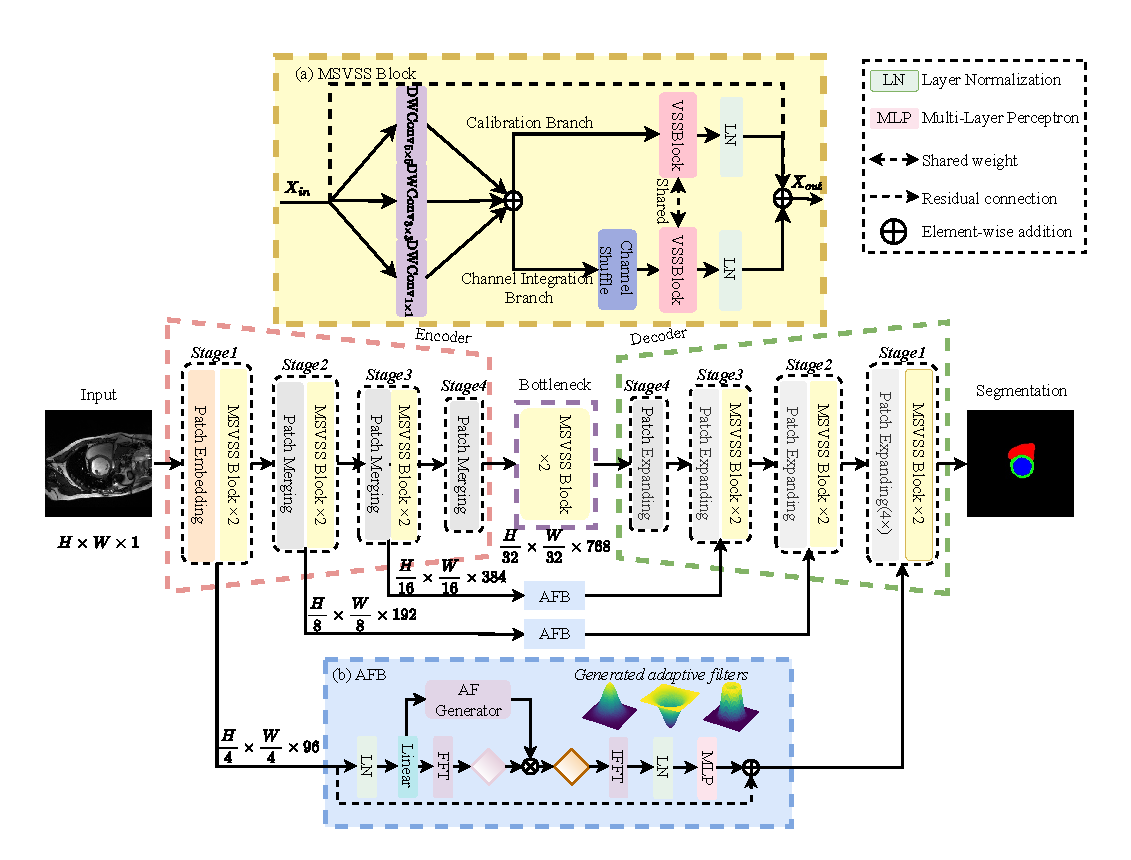
\includegraphics[width=0.95\textwidth]{paper/model_new.pdf}
    \fbox{\parbox{0.75\textwidth}{\centering\vspace{3cm}图3-1 占位：SAF-Mamba整体架构与MSVSS、AFB模块\\（可替换为paper/model\_new.pdf）\vspace{3cm}}}
    \caption{SAF-Mamba整体架构与MSVSS、AFB模块示意图}
    \label{fig:safmamba}
\end{figure}

\subsection{实验与分析}

\subsubsection{实验数据与预处理}

实验在ACDC与M\&Ms两个心脏分割数据集上进行。ACDC包含100名患者的200例标注心脏MRI扫描，标注右心室（RV）、心肌（MYO）和左心室（LV），按70例训练、10例验证、20例测试划分，共1930张训练切片。M\&Ms包含来自四个厂商（Siemens、Philips、GE、Canon）的375名患者、7334张标注切片，训练集为150例标注扫描，厂商C的25例未标注扫描被排除，测试集为每厂商50例共200例。数据预处理遵循Mamba-UNet与UTNet的设置，ACDC输入尺寸为$224 \times 224$，M\&Ms为$256 \times 256$，采用归一化及常规数据增强。

\subsubsection{评价指标}

采用Dice相似系数（DSC）与95\%豪斯多夫距离（HD95）作为主要评价指标。DSC衡量预测与真实分割的重叠程度，取值范围$[0,1]$，越高越好；HD95衡量边界误差，单位为毫米，越低越好。

\subsubsection{实验设置}

实验在单张16GB NVIDIA RTX 3090 GPU上进行，使用PyTorch 2.1.1。ACDC训练15000次迭代，M\&Ms训练10000次迭代，批大小为16。优化器为SGD，学习率0.01，动量0.9。损失函数为交叉熵与Dice损失的组合。

\subsubsection{对比实验}

表\ref{tab:acdc_sa}与表\ref{tab:mms_sa}分别展示了引入多尺度感知模块的初步网络模型 SA-Mamba 在ACDC与M\&Ms上的对比结果。SA-Mamba在ACDC上取得了91.25\%的平均DSC与1.47 mm的HD95，在RV与MYO分割精度上已有显著提升。在M\&Ms上取得平均DSC 87.35\% 与 HD95 12.86 mm，展现出比基础 Mamba-UNet 更好的适应能力，初步验证了MSVSS模块在应对多尺度挑战时的有效性。完整模型的综合冲顶对比将在第四章展示。

\begin{table}[H]
    \centering
    \caption{ACDC数据集 SA-Mamba 对比实验初步结果}
    \label{tab:acdc_sa}
    \begin{tabular}{cccccc}
        \toprule
        \multirow{2}{*}{方法} & \multicolumn{4}{c}{DSC(\%)$\uparrow$} & \multirow{2}{*}{HD95(mm)$\downarrow$} \\
        & RV & MYO & LV & Avg & \\
        \midrule
        U-Net & 85.01 & 86.35 & 94.29 & 88.55 & 2.39 \\
        TransUNet & 86.87 & 84.22 & 94.12 & 88.40 & 1.65 \\
        Mamba-UNet & 90.25 & 88.39 & 94.27 & 90.97 & 1.81 \\
        \midrule
        \textbf{SA-Mamba(本文)} & \textbf{90.54} & \textbf{88.75} & \textbf{94.46} & \textbf{91.25} & \textbf{1.47} \\
        \bottomrule
    \end{tabular}
\end{table}

\begin{table}[H]
    \centering
    \caption{M\&Ms数据集 SA-Mamba 对比实验初步结果}
    \label{tab:mms_sa}
    \begin{tabular}{ccccccc}
        \toprule
        \multirow{2}{*}{方法} & \multicolumn{5}{c}{DSC(\%)$\uparrow$} & \multirow{2}{*}{HD95(mm)$\downarrow$} \\
        & A & B & C & D & Avg & \\
        \midrule
        U-Net & 87.65 & 84.80 & 82.69 & 83.79 & 84.73 & 15.85 \\
        TransUNet & 87.69 & 85.82 & 84.25 & 85.53 & 85.82 & 13.30 \\
        Mamba-UNet & 88.32 & 86.48 & 83.11 & 86.98 & 86.22 & 14.05 \\
        \midrule
        \textbf{SA-Mamba(本文)} & \textbf{88.85} & \textbf{87.12} & \textbf{84.55} & \textbf{88.88} & \textbf{87.35} & \textbf{12.86} \\
        \bottomrule
    \end{tabular}
\end{table}

\subsubsection{分割结果的可视化分析}

定性可视化表明，得益于多尺度特征的整合，SA-Mamba在处理不同大小心腔结构时相较于基线模型展现出明显优势。与Mamba-UNet相比，引入MSVSS后的SA-Mamba在右心室等小尺度靶区的分割上表现更为稳定，初步缓解了尺度极差带来的漏分现象。然而，受限于单纯的空间域特征提取，在心肌与左心室交界等极其模糊的区域，其边界平滑度仍存在瑕疵。这些遗留的边界问题，将由第四章完整加入AFB后的SAF-Mamba彻底解决，相关深层次对比可视化见第四章分析。

\subsection{本章小结}

本章介绍了MSVSS模块的设计思想与实现细节，包括并行多尺度深度卷积分支、通道整合与校准机制以及共享VSS的特征提取。基于MSVSS构建的SA-Mamba网络在ACDC与M\&Ms数据集上取得了优于现有方法的性能，验证了多尺度感知策略对心脏分割中尺度变化挑战的有效应对能力。

%%%%%%%%%%%%%%% 第四章 基于自适应d滤波的边界细化方法 %%%%%%%%%%%%%%%
\reSection{第四章\quad 基于自适应频域滤波的医学图像分割}

虽然第三章提出的多尺度视觉状态空间（MSVSS）模块通过空间维度的特征聚合，有效捕捉了不同尺度目标的上下文信息，缓解了器官尺度多样性的问题；然而，在编码器的逐层下采样（池化或步进卷积）过程中，图像的高频细节（如边界轮廓、微小组织结构）势必会发生严重衰减。单靠空间维度的特征提取难以从根本上挽回这些已经丢失的高频信息。

基于这一严峻的挑战，本章从频率域视角出发，引入自适应频域滤波模块（AFB），通过在频域进行有区分度的特征增强，找回并细化丢失的边界。本章将详细阐述 AFB 的设计原理，并通过消融实验及与现有先进方法的综合对比，全面验证完整模型 SAF-Mamba 的最终性能。

\subsection{下采样过程中的高频信息丢失问题}

在编码器-解码器结构中，下采样操作在降低空间分辨率的同时，会不可避免地衰减高频分量。根据傅里叶分析，高频对应边缘、纹理等细节，低频对应整体轮廓与平滑区域。高频信息的丢失导致解码器恢复的边界模糊、定位不准，影响分割精度。因此，在跳跃连接中对编码器特征进行频域增强，有助于在融合到解码器时保留更多边界细节，提升边界贴合度与平滑度。

\subsection{自适应滤波器模块}

AFB对跳跃连接中的编码器特征进行自适应频域滤波。设空间特征$\mathbf{X}_i \in \mathbb{R}^{H \times W \times C}$，经层归一化（Layer Normalization, LN）与线性层投影至$\hat{\mathbf{X}}_i \in \mathbb{R}^{H \times W \times 2C}$，再经2D FFT变换至频域。根据先验工作，2D DFT可将空间信号分解为频率分量；为加速计算，采用2D FFT实现。自适应滤波器由AF Generator根据输入特征动态生成，在频域中与特征逐元素相乘，增强有效频率、抑制噪声，最后经IFFT重构至空间域：
\begin{equation}
A(\hat{\mathbf{X}}_i) = \mathcal{F}^{-1}\left( \mathcal{F}(\hat{\mathbf{X}}_i) \odot \mathbf{F}_c \right)
\end{equation}
其中$\odot$表示逐元素乘法，$\mathcal{F}(\cdot)$与$\mathcal{F}^{-1}(\cdot)$分别为2D FFT与IFFT，$\mathbf{F}_c$为AF Generator生成的滤波器，根据输入特性调制频谱。经MLP建模跨通道依赖并精炼特征后，通过残差融合得到最终输出$\mathbf{X}_i^{out} \in \mathbb{R}^{H \times W \times C}$，恢复空间细节。

\subsubsection{自适应滤波器生成器}

AF Generator是AFB的核心组件，其作用是根据输入特征的内容动态生成滤波器参数，使滤波行为随输入自适应变化。与固定高通、低通或带通滤波器不同，AF Generator生成的滤波器可根据不同区域、不同阶段的需求，呈现高通（增强边界）、低通（平滑噪声）或带通（保留特定频段）等多样化模式。这种自适应性使得AFB能够在不增加大量参数的前提下，灵活应对医学图像中边界与噪声的复杂分布。

AF Generator通过MLP与Softmax归一化产生通道级权重，对滤波器基$\mathbb{M} = \{\mathcal{M}_1, \ldots, \mathcal{M}_N\}$进行线性组合，其中每个$\mathcal{M}_i \in \mathbb{C}^{H \times \lceil W/2 \rceil}$为随机初始化的复参数。由于各频谱通道对应不同频率响应，采用逐通道滤波。权重计算为：
\begin{equation}
\mathbf{a} = \text{Softmax}\left( \text{MLP}\left( \frac{\sum_{h=1}^{H}\sum_{w=1}^{W} \mathbf{X}_{:,h,w}}{HW} \right) \right)
\end{equation}
\begin{equation}
\mathbf{a} = (\alpha_1, \ldots, \alpha_{N \cdot 2C})^\top
\end{equation}
自适应滤波器由下式生成：
\begin{equation}
\mathbf{F}_c = \sum_{i=1}^{N} \frac{e^{\alpha_{c,i}}}{\sum_{n=1}^{N} e^{\alpha_{c,n}}} \mathcal{M}_i
\end{equation}
其中$\alpha_{c,i}$为第$c$组$\alpha$的第$i$个元素，$\alpha$被划分为$N$段，每段长度$2C$。本文设置$N=3$。$N$过大增加计算成本，$N$过小（如$N=1$）则滤波器退化为固定形式，失去自适应性。

\subsubsection{频域调制与特征重构}

生成的滤波器$\mathbf{F}_c$在频域中与$\mathcal{F}(\hat{\mathbf{X}}_i)$逐元素相乘，实现对特定频率（尤其是高频细节）的自适应增强。根据输入内容，滤波器可呈现高通、低通或带通特性，在边界区域往往呈现高通特性以增强边缘。经IFFT将调制后的频谱重构回空间域，得到增强后的特征，再经MLP与残差融合，输出最终特征供解码器使用。

\subsection{实验与分析}

\subsubsection{实验设置}

本章实验与第三章共享数据、评价指标及大部分超参数设置。消融实验中，基线为Mamba-UNet（即无MSVSS、无AFB），逐步添加MSVSS、AFB或两者，以验证各模块贡献。

\subsubsection{对比实验}

为验证完整SAF-Mamba模型在心脏图像分割任务上的优异性能，本节展示其与现有各类先进网络在ACDC与M\&Ms数据集上的全面对比结果。如表\ref{tab:acdc_full}与表\ref{tab:mms_full}所示，得益于频域AFB模块与空间域MSVSS模块的强强联合，完整版SAF-Mamba在ACDC上取得最高平均DSC（92.21\%）与最低HD95（1.05 mm），显著优于单纯的Swin-Unet、HiFormer以及基础版本的Mamba-UNet等对比方法。在M\&Ms跨厂商数据集上，SAF-Mamba同样取得最佳评价指标，充分验证了模型强大的鲁棒性与广泛的泛化潜力。

\begin{table}[H]
    \centering
    \caption{ACDC数据集 SAF-Mamba 综合对比实验结果}
    \label{tab:acdc_full}
    \begin{tabular}{cccccc}
        \toprule
        \multirow{2}{*}{方法} & \multicolumn{4}{c}{DSC(\%)$\uparrow$} & \multirow{2}{*}{HD95(mm)$\downarrow$} \\
        & RV & MYO & LV & Avg & \\
        \midrule
        U-Net & 85.01 & 86.35 & 94.29 & 88.55 & 2.39 \\
        Swin-Unet & 85.62 & 84.49 & 94.03 & 88.05 & 2.08 \\
        TransUNet & 86.87 & 84.22 & 94.12 & 88.40 & 1.65 \\
        HiFormer & 90.51 & 89.27 & 95.68 & 91.82 & 1.12 \\
        TransCASCADE & 89.07 & 88.90 & 94.45 & 90.81 & 1.29 \\
        PVT-CASCADE & 90.15 & 89.97 & 95.05 & 91.72 & 1.16 \\
        Swin-UMamba & 85.12 & 83.73 & 93.81 & 87.55 & 2.47 \\
        UU-mamba & 90.23 & 89.43 & 95.60 & 91.75 & 1.20 \\
        Mamba-UNet & 90.25 & 88.39 & 94.27 & 90.97 & 1.81 \\
        \midrule
        \textbf{SAF-Mamba(本文)} & \textbf{90.87} & \textbf{89.42} & \textbf{96.34} & \textbf{92.21} & \textbf{1.05} \\
        \bottomrule
    \end{tabular}
\end{table}

\begin{table}[H]
    \centering
    \caption{M\&Ms数据集 SAF-Mamba 综合对比实验结果}
    \label{tab:mms_full}
    \begin{tabular}{ccccccc}
        \toprule
        \multirow{2}{*}{方法} & \multicolumn{5}{c}{DSC(\%)$\uparrow$} & \multirow{2}{*}{HD95(mm)$\downarrow$} \\
        & A & B & C & D & Avg & \\
        \midrule
        U-Net & 87.65 & 84.80 & 82.69 & 83.79 & 84.73 & 15.85 \\
        Swin-Unet & 86.27 & 84.52 & 83.11 & 84.95 & 84.71 & 13.66 \\
        TransUNet & 87.69 & 85.82 & 84.25 & 85.53 & 85.82 & 13.30 \\
        HiFormer & 87.90 & 83.94 & 83.25 & 83.86 & 84.74 & 12.78 \\
        TransCASCADE & 85.92 & 84.23 & 82.93 & 84.43 & 84.38 & 13.91 \\
        PVT-CASCADE & 88.71 & 87.12 & 85.36 & 87.81 & 87.25 & 12.60 \\
        Swin-UMamba & 87.88 & 86.15 & 83.67 & 85.28 & 85.75 & 13.29 \\
        UU-mamba & 88.15 & 86.90 & 85.22 & 86.79 & 86.77 & 13.09 \\
        Mamba-UNet & 88.32 & 86.48 & 83.11 & 86.98 & 86.22 & 14.05 \\
        \midrule
        \textbf{SAF-Mamba(本文)} & \textbf{89.16} & \textbf{88.79} & \textbf{86.83} & \textbf{88.92} & \textbf{88.43} & \textbf{12.14} \\
        \bottomrule
    \end{tabular}
\end{table}

\subsubsection{消融实验}

表\ref{tab:ablation}展示了在ACDC上的消融结果。移除MSVSS或AFB均导致性能下降，表明二者具有互补作用。同时集成两者时，SAF-Mamba取得最高DSC（92.21\%）与最低HD95（1.05 mm），验证了MSVSS与AFB联合使用的有效性。

\begin{table}[H]
    \centering
    \caption{ACDC数据集消融实验结果}
    \label{tab:ablation}
    \begin{tabular}{ccccc}
        \toprule
        方法 & MSVSS & AFB & DSC(\%)$\uparrow$ & HD95(mm)$\downarrow$ \\
        \midrule
        \multirow{4}{*}{SAF-Mamba(本文)} & $\times$ & $\times$ & 90.97 & 1.81 \\
        & $\checkmark$ & $\times$ & 91.25 & 1.47 \\
        & $\times$ & $\checkmark$ & 91.54 & 1.42 \\
        & $\checkmark$ & $\checkmark$ & 92.21 & 1.05 \\
        \bottomrule
    \end{tabular}
\end{table}

\subsubsection{自适应滤波器基的频域可视化分析}

将不同病例或不同区域的图像块输入AF Generator，对生成的滤波器参数进行可视化，可直观展示滤波器如何根据输入内容自适应调整。实验表明，学习到的滤波器在不同阶段呈现多样化的高通、低通与带通模式，验证了AFB的自适应频域调制能力。


除DSC与HD95外，可引入针对边界的评价指标如平均对称表面距离（Average Symmetric Surface Distance, ASSD）进行补充评估。通过放大分割结果的边界区域进行可视化对比，可定性展示加入AFB后边界的贴合度与平滑度改善。HD95的显著降低（从1.81 mm至1.05 mm）也定量印证了AFB对边界精度的提升。

\subsubsection{基于皮肤病灶分割的泛化能力验证}

为验证SAF-Mamba对不同模态、不同任务的泛化能力，可在ISIC2017等皮肤病灶分割数据集上进行实验，将完整SAF-Mamba与任务相关SOTA方法对比。该部分可根据实际实验进度补充表格与图示。

\subsection{本章小结}

本章介绍了AFB模块的设计思想与实现细节，包括FFT/IFFT的频域变换、AF Generator的自适应滤波器生成以及频域调制与特征重构流程。消融实验与可视化分析表明，AFB能有效增强边界细节；结合MSVSS，完整集成的SAF-Mamba模型在心脏分割任务上具备良好的综合性能与泛化能力。

%%%%%%%%%%%%%%% 第五章 总结与展望 %%%%%%%%%%%%%%%
\reSection{第五章\quad 总结与展望}

\subsection{工作总结}

本文针对医学图像分割中的尺度变化与边界模糊两大共性挑战，提出了基于多尺度状态空间模型和自适应频率滤波的SAF-Mamba模型，主要工作可总结如下：

（1）设计了多尺度视觉状态空间（MSVSS）模块，通过并行多尺度深度卷积分支、通道整合与校准机制，有效捕获不同尺度目标的特征表示，增强模型对尺度变化的敏感性。MSVSS模块与共享VSS的联合设计在保证多尺度感知能力的同时，兼顾了计算效率。

（2）构建了自适应滤波器模块（AFB），利用FFT将编码器跳跃连接特征映射至频域，通过AF Generator根据输入内容动态生成滤波器参数，在频域中调制频率分量以增强边界细节，最后经IFFT重构空间特征。AFB能够自适应呈现高通、低通或带通特性，有效缓解下采样过程中的高频信息丢失。

（3）将MSVSS与AFB集成于U型编码器-解码器架构，形成完整的SAF-Mamba网络。在ACDC与M\&Ms心脏分割数据集上，SAF-Mamba取得了优于CNN、Transformer及Mamba类现有方法的性能，验证了方法的有效性与高泛化能力。

（4）提出核心理论范式：本研究打破了现有视觉状态空间模型高度依赖空间域特征提取的局限，为 Mamba 架构在密集预测任务中实现“空间大感受野统筹”与“高频精准边界保留”的协同处理提供了一种全新范式。这一理论视角的补充，显著提升了模型表现，更为医学图像分割领域的创新提供了具有更强鲁棒性与泛化能力的网络设计思路。

\subsection{未来展望}

基于本文研究的发现与局限性，未来可从以下方向开展进一步工作：

（1）\textbf{模型轻量化}：当前SAF-Mamba在精度上表现优异，但模型规模与计算开销对临床部署（如移动端、嵌入式设备）仍有一定限制。未来可探索知识蒸馏、模型剪枝、量化等技术，在保持性能的同时降低计算与存储开销，便于在资源受限场景下的实际应用。

（2）\textbf{向3D/4D扩展}：本文方法基于2D切片，而医学影像常以3D体积或4D动态序列形式存在。将MSVSS与AFB扩展至3D乃至4D数据，可更充分利用空间与时间上下文，处理CT、MRI体积数据及心脏动态序列等更复杂的医学数据。

（3）\textbf{与SAM及大模型方向的结合}：Segment Anything Model（SAM）等基础模型在零样本与少样本分割上展现出强大能力，其提示式（Prompt-based）分割范式与医学图像分割的交互式标注需求高度契合；视觉大模型（Vision Large Language Model, VLLM）在理解与推理方面具有独特优势，可提供高层语义先验。未来可探索将SAF-Mamba与SAM或大模型相结合，如利用SAM的提示机制增强边界定位，或借助大模型的语义理解能力提升复杂场景下的分割一致性，形成“小模型+大模型”的协同框架，以应对标注数据稀缺与长尾类别等实际挑战。

\subsection{本章小结}

本章对全文研究工作进行了系统总结，梳理了SAF-Mamba模型在医学图像分割中的三项核心贡献：多尺度视觉状态空间模块的设计、自适应频域滤波模块的构建，以及二者在完整网络框架中的协同集成。同时，从模型轻量化、三维扩展以及与基础大模型结合三个维度对未来研究方向进行了展望，以期为后续工作提供参考与借鉴。

%%%%%%%%%%%%%%% 参考文献 %%%%%%%%%%%%%%%
\section*{参考文献}
\reference{
    \bibitem{1} Ronneberger O, Fischer P, Brox T. U-net: Convolutional networks for biomedical image segmentation[C]//Medical Image Computing and Computer-Assisted Intervention--MICCAI 2015. Springer, 2015: 234-241.
    \bibitem{2} Cao H, Wang Y, Chen J, et al. Swin-unet: Unet-like pure transformer for medical image segmentation[C]//European Conference on Computer Vision. Springer, 2022: 205-218.
    \bibitem{3} Dosovitskiy A, Beyer L, Kolesnikov A, et al. An image is worth 16x16 words: Transformers for image recognition at scale[J]. arXiv preprint arXiv:2010.11929, 2021.
    \bibitem{4} Gu A, Dao T. Mamba: Linear-time sequence modeling with selective state spaces[J]. arXiv preprint arXiv:2312.00752, 2023.
    \bibitem{5} Gu A, Goel K, Ré C. Efficiently modeling long sequences with structured state spaces[J]. arXiv preprint arXiv:2111.00396, 2022.
    \bibitem{6} Liu Y, Tian Y, Zhao Y, et al. VMamba: Visual state space model[J]. arXiv preprint arXiv:2401.10166, 2024.
    \bibitem{7} Ma M, Xia C, Xie C, et al. Boosting broader receptive fields for salient object detection[J]. IEEE Transactions on Image Processing, 2023, 32: 1026-1038.
    \bibitem{8} Rahman M M, Munir M, Marculescu R. EMCAD: Efficient multi-scale convolutional attention decoding for medical image segmentation[C]//Proceedings of the IEEE/CVF Conference on Computer Vision and Pattern Recognition. 2024: 11769-11779.
    \bibitem{9} Zhang X, Zhou X, Lin M, et al. Shufflenet: An extremely efficient convolutional neural network for mobile devices[C]//Proceedings of the IEEE Conference on Computer Vision and Pattern Recognition. 2018: 6848-6856.
    \bibitem{10} Tatsunami Y, Taki M. FFT-based dynamic token mixer for vision[C]//Proceedings of the AAAI Conference on Artificial Intelligence. 2024, 38(14): 15328-15336.
    \bibitem{11} Chang A, Zeng J, Huang R, et al. EM-Net: Efficient channel and frequency learning with Mamba for 3D medical image segmentation[C]//International Conference on Medical Image Computing and Computer-Assisted Intervention. Springer, 2024: 266-275.
    \bibitem{12} Bernard O, Lalande A, Zotti C, et al. Deep learning techniques for automatic MRI cardiac multi-structures segmentation and diagnosis: Is the problem solved?[J]. IEEE Transactions on Medical Imaging, 2018, 37(11): 2514-2525.
    \bibitem{13} Campello V M, Gkontra P, Izquierdo C, et al. Multi-centre, multi-vendor and multi-disease cardiac segmentation: The M\&Ms challenge[J]. IEEE Transactions on Medical Imaging, 2021, 40(12): 3543-3554.
    \bibitem{14} Wang Z, Zheng J-Q, Zhang Y, et al. Mamba-UNet: UNet-like pure visual Mamba for medical image segmentation[J]. arXiv preprint arXiv:2402.05079, 2024.
    \bibitem{15} Gao Y, Zhou M, Metaxas D N. UTNet: A hybrid transformer architecture for medical image segmentation[C]//Medical Image Computing and Computer Assisted Intervention--MICCAI 2021. Springer, 2021: 61-71.
    \bibitem{16} Chen J, Lu Y, Yu Q, et al. TransUNet: Transformers make strong encoders for medical image segmentation[J]. arXiv preprint arXiv:2102.04306, 2021.
    \bibitem{17} Heidari M, Kazerouni A, Soltany M, et al. HiFormer: Hierarchical multi-scale representations using transformers for medical image segmentation[C]//Proceedings of the IEEE/CVF Winter Conference on Applications of Computer Vision. 2023: 6202-6212.
    \bibitem{18} Rahman M M, Marculescu R. Medical image segmentation via cascaded attention decoding[C]//2023 IEEE/CVF Winter Conference on Applications of Computer Vision. IEEE, 2023: 6211-6220.
    \bibitem{19} Liu J, Yang H, Zhou H-Y, et al. Swin-UMamba: Mamba-based UNet with ImageNet-based pretraining[C]//International Conference on Medical Image Computing and Computer-Assisted Intervention. Springer, 2024: 615-625.
    \bibitem{20} Tsai T Y, Lin L, Hu S, et al. UU-Mamba: Uncertainty-aware U-Mamba for cardiac image segmentation[J]. arXiv preprint arXiv:2405.17496, 2024.
}

%%%%%%%%%%%%%%% 致谢 %%%%%%%%%%%%%%%
\reThanks{
    本论文的完成离不开导师的悉心指导和实验室同门的无私帮助。

    首先，衷心感谢导师在选题、方法设计、实验分析与论文撰写全过程中的指导与支持。导师严谨的治学态度与渊博的专业知识使我受益良多。

    其次，感谢实验室同门在学术交流与技术讨论中给予的启发与帮助，感谢他们在实验环境与代码实现上的支持。

    最后，感谢家人一直以来的理解与鼓励，他们的支持是我完成学业的坚强后盾。
}

\end{document}
